%! TeX program = lualatex
\documentclass[../main.tex]{subfiles}
\begin{document} \section{Derivatives (as functions)}
% Do change of variable.

\begin{mdframed}[style=withref]
  \textbf{Definition}. The \emph{derivative} of a \(f(x)\) as a function, denoted by \(f'(x)\), is
  \begin{equation} \label{eq:derivative}
    f'(x) = {\lim_{h \to 0} \frac{f(x+h) - f(x)}{h}}
  \end{equation}
  The function \(f'(x)\) is defined wherever the limit in Equation~\eqref{eq:derivative} exists.

  \textbook{Page 232}
\end{mdframed}
\textbf{Terminologies}. Let \(f(x)\) be a function and \(a\) be a number.
\begin{itemize}
  \item ``Differentiate \(f\) (with respect to \(x\))'' means \underline{\hspace{3in}}
  \item ``\(f(x)\) is differentiable at \(a\)'' means \underline{\hspace{3.62in}}
  \item ``\(f(x)\) is differentiable on \((a,b)\)'' means \underline{\hspace{3.36in}}
\end{itemize}

\bigskip
\begin{example}
  Let \(f(x) = \sqrt{x + 1}\). Find a formula for \(f'\) from definition (meaning use Equation~\eqref{eq:derivation}) and determine the domain of \(f'\).

  \blanklines{32}
\end{example}

\clearpage

\textbf{Notations}. If we write \(y = f(x)\) to denote a function, then \emph{all} of the following denote the function that is the derivative of \(f(x)\).
\[
  f'(x) 
  \;=\; f' 
  \;=\; y' 
  \qquad =\qquad  
  {\color{main} \frac{d}{dx}} \, f(x) \;=\; \frac{df}{dx} \;=\; \frac{dy}{dx}
  \qquad=\quad 
  Df(x) 
  \;=\; D_{x} f(x)
\]

\emph{All} of the following denote the derivative of \(f(x)\) at a number \(a\).
\begin{align*}
  & f'(a) \quad=\quad \frac{dy}{dx} \bigg|_{x = a} \quad=\quad \frac{dy}{dx} \bigg]_{x = a}
\end{align*}

\label{page:higher-derivatives}
In general, we define \(f^{(0)} = f\) and the \(n\)-th derivative to be
\[
  \overbrace{f^{' \cdots '}}^{\text{\(n\) primes}} \quad=\quad f^{(n)} \quad=\quad \frac{d^{n}}{dx^{n}} f \quad=\quad \frac{d}{dx} f^{(n-1)} \quad\text{for integers } n \ge 1.
\]

\begin{example}
  Find the second derivative of \(x^{2}\) from the definition (use Equation~\eqref{eq:derivative}).

  \blanklines{30}
\end{example}

\begin{example}
  Suppose \(s(t)\) is the displacement function of some object. What is the physical interpretation of \(s''(t)\)?

  \blanklines{5}
\end{example}
\clearpage

\begin{example}
  Use the graph of \(f(x)\) to sketch its derivative. 

  \begin{center}
    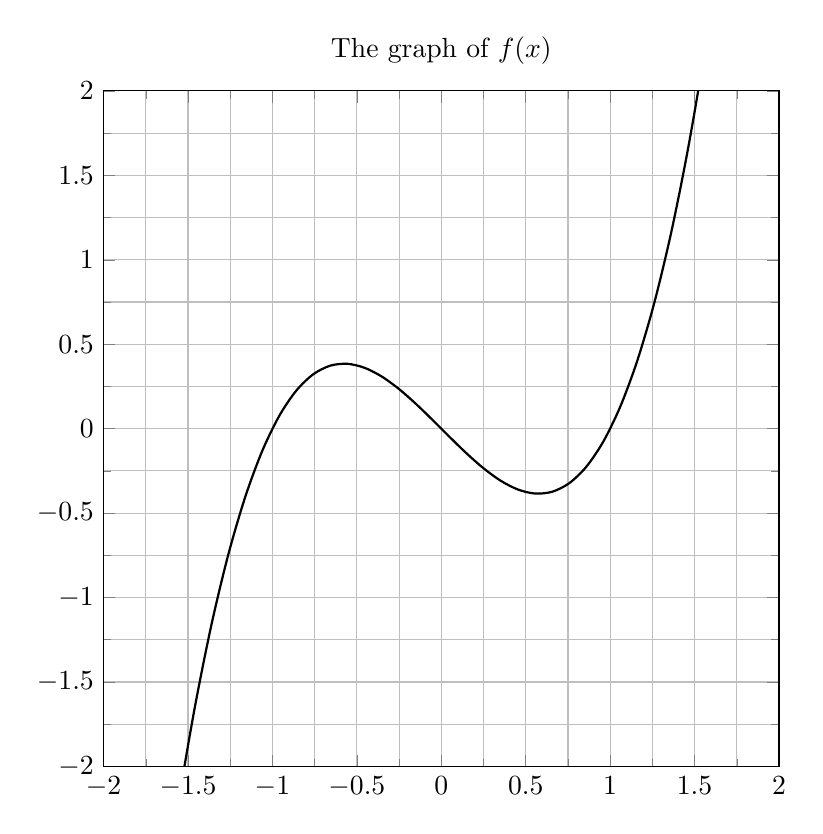
\begin{tikzpicture}
      \begin{axis}[width=4in, height=4in, smooth, samples=100, grid=both, minor tick num=1, ymin=-2,ymax=2, xmin=-2, xmax=2, axis equal, title={The graph of \(f(x)\)}
        ]
        \addplot[thick, black] {x^3 - x};
        % \node[right] (axis cs:1.5,1) {\footnotesize \(f'(x)\)};
      \end{axis}
    \end{tikzpicture}  

    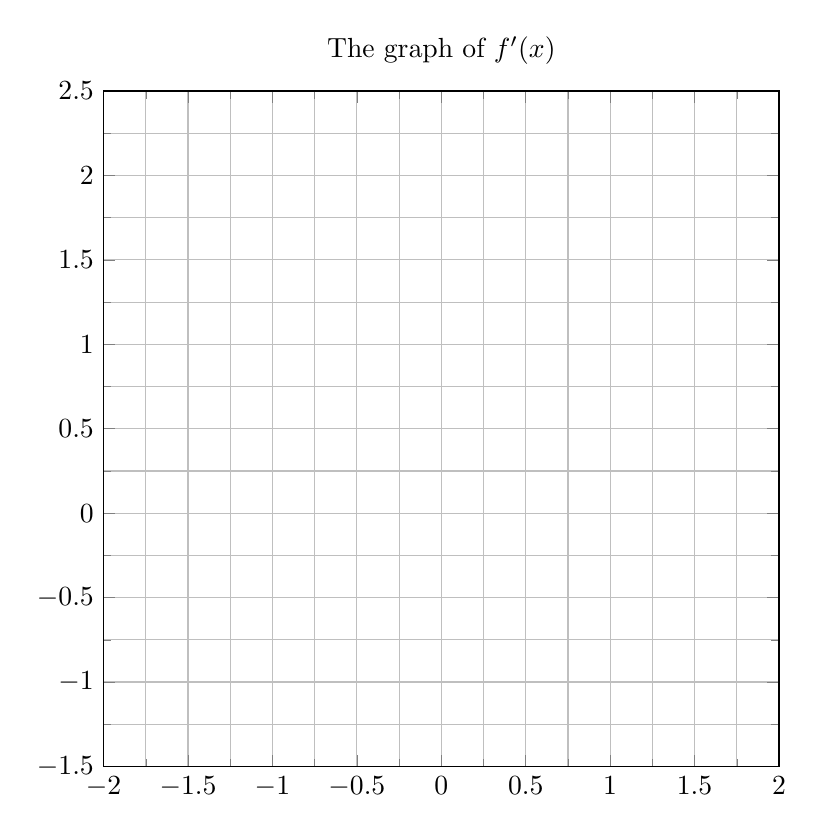
\begin{tikzpicture}
      \begin{axis}[width=4in, height=4in, smooth, samples=100, grid=both, minor tick num=1, ymin=-1.5,ymax=2.5, xmin=-2, xmax=2, axis equal, title={The graph of \(f'(x)\)}
        ]
        % \addplot[thick, black] {3*x^2 - 1};
      \end{axis}
    \end{tikzpicture}  
  \end{center}
\end{example}
\clearpage

\begin{example}
  The derivative of a function \(f\) is \(x+1\) and \(f\) passes through \((1, 2)\). Sketch the tangent line of \(f\) at \(x = 1\). 

  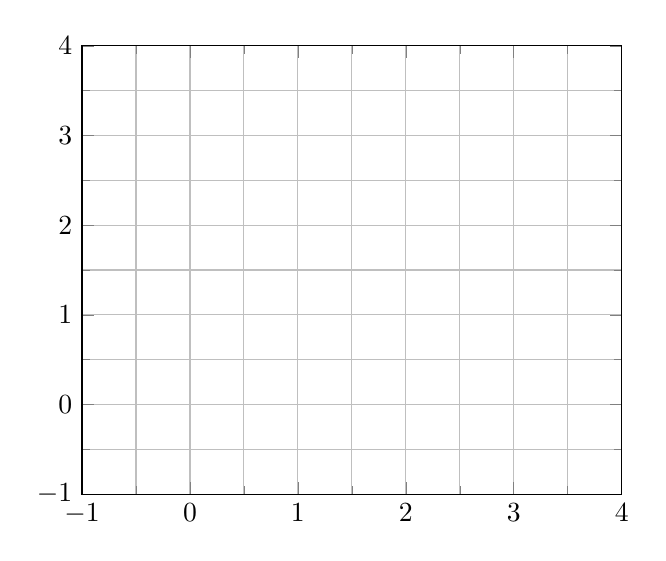
\begin{tikzpicture}
    \begin{axis}[xmin=-1, xmax=4, ymin=-1, ymax=4, grid=both, minor tick num=1]
      
    \end{axis}
  \end{tikzpicture}


  For an extra challenge, approximate a root of \(f\) by sketching \(f\) without trying to guess the function \(f\) or doing any integration even if you know that sort of dark magic.  If you are able to do so using only the derivative and \(f(1) = 2\), then you have reinvented the mathematical foundation of modern machine learning. A very early form of this method was written in 1669 and is often attributed to Sir Issac Newton.

  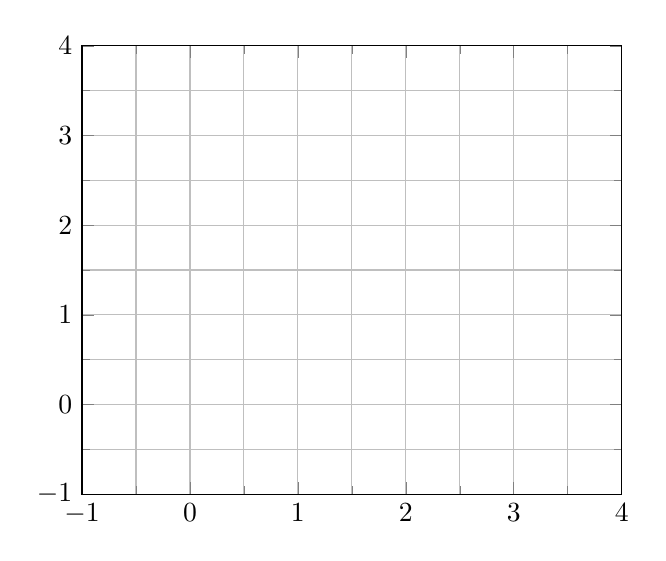
\begin{tikzpicture}
    \begin{axis}[xmin=-1, xmax=4, ymin=-1, ymax=4, grid=both, minor tick num=1]
      
    \end{axis}
  \end{tikzpicture}
\end{example}

\end{document}

